\documentclass[11pt,letterpaper]{article}
\usepackage[T1]{fontenc}
\usepackage[utf8]{inputenc}
\usepackage[margin=1in,headheight=15pt]{geometry}
\usepackage{microtype}
\usepackage{amsmath,amsthm,mathtools}
\usepackage{newtxtext,newtxmath}
\usepackage{booktabs,tabularx,array,longtable}
\usepackage{enumitem}
\usepackage{algorithm,algpseudocode}
\usepackage{listings}
\usepackage{xcolor}
\usepackage{tikz}
\usetikzlibrary{arrows.meta,positioning,fit,calc}
\usepackage{natbib}
\setcitestyle{authoryear,square,comma}
\usepackage{xurl}
\usepackage[hidelinks,unicode]{hyperref}
\usepackage{fancyhdr,titlesec,needspace,caption}
\hypersetup{pdftitle={Transformational Intelligence: Learning to Change the Game},pdfauthor={Vincent Boucher},pdfsubject={Discovering and demonstrating better problem formulations},pdfkeywords={transformational intelligence, problem formulation, conceptual spaces, causal experimentation, meta-strategic intelligence, evidence}}
\pagestyle{fancy}\fancyhf{}
\fancyhead[L]{\small Transformational Intelligence}
\fancyhead[R]{\small Boucher}
\fancyfoot[C]{\thepage}
\renewcommand{\headrulewidth}{0.3pt}
\setlength{\parindent}{1.1em}
\setlength{\parskip}{0.23em}
\setlength{\emergencystretch}{2em}
\linespread{1.04}
\titleformat{\section}{\large\bfseries}{\thesection}{0.6em}{}
\titleformat{\subsection}{\normalsize\bfseries}{\thesubsection}{0.6em}{}
\titlespacing*{\section}{0pt}{2.3ex plus .8ex minus .2ex}{0.8ex plus .2ex}
\titlespacing*{\subsection}{0pt}{1.6ex plus .5ex minus .2ex}{0.4ex plus .2ex}
\captionsetup{font=small,labelfont=bf}
\setlist{nosep,leftmargin=1.5em,topsep=0.3em}
\renewcommand{\topfraction}{.93}\renewcommand{\bottomfraction}{.85}
\renewcommand{\textfraction}{.06}\renewcommand{\floatpagefraction}{.8}
\newcolumntype{Y}{>{\raggedright\arraybackslash}X}
\newcolumntype{P}[1]{>{\raggedright\arraybackslash}p{#1}}
\newcommand{\E}{\mathbb E}
\newcommand{\Prob}{\mathbb P}
\newcommand{\I}{\mathcal I}
\newcommand{\D}{\mathcal D}
\newcommand{\A}{\mathcal A}
\newcommand{\Fset}{\mathfrak F}
\newcommand{\Hist}{\mathcal H}
\newcommand{\ind}{\mathbf 1}
\DeclareMathOperator*{\argmin}{arg\,min}
\DeclareMathOperator*{\argmax}{arg\,max}
\newtheorem{definition}{Definition}[section]
\newtheorem{proposition}{Proposition}[section]
\newtheorem{theorem}{Theorem}[section]
\newtheorem{corollary}{Corollary}[section]
\theoremstyle{remark}\newtheorem{remark}{Remark}[section]
\newcommand{\thesisbox}[1]{\begin{center}\fbox{\begin{minipage}{0.94\linewidth}\vspace{.35em}#1\vspace{.35em}\end{minipage}}\end{center}}
\lstset{basicstyle=\small\ttfamily,breaklines=true,columns=fullflexible,keepspaces=true,showstringspaces=false,frame=single,rulecolor=\color{black!30},aboveskip=.7em,belowskip=.7em}
\begin{document}
\thispagestyle{plain}
\begin{center}
{\fontsize{26}{30}\selectfont\bfseries Transformational Intelligence\par}
\vspace{.35em}
{\Large Learning to Change the Game\par}
\vspace{1.05em}
{\large Vincent Boucher\par}
{MONTREAL.AI\par}
{Montr\'eal, Qu\'ebec, Canada\par}
\vspace{.65em}
{October 2026\quad$\cdot$\quad Research manuscript\par}
\end{center}
\vspace{.1em}
\begin{abstract}
An AI can search more effectively while remaining trapped in an unnecessarily restrictive problem formulation. More computation cannot recover information absent from every allowed observation; better scheduling cannot remove dependencies that the workflow itself imposes. We develop \emph{transformational intelligence}: the capacity to identify such restrictions, invent a different problem-solving setup, and demonstrate that the change better serves an authorized purpose. The object of invention is a formulation---its representations, assumptions, information channels, coordination rules, and intermediate objectives---not only an answer or a strategy within it. We separate intended outcomes from inherited means and from the instruments used to measure success. A transformation must carry an executable realization, a bridge back to the intended outcome, and evidence that the proposed structural change matters. An exact, reproducible causal-identification study illustrates the distinction: every passive procedure is limited to $50\%$ accuracy under the specified model, whereas an intervention policy reaches $8191/8192$ accuracy with at most twelve queries. A standard unrestricted optimal planner matches this policy; the result demonstrates a formulation-dependent limit, not a new causal-discovery algorithm or an LLM achievement. We then specify an architecture for discovering transformations, including complementary changes that fail in isolation, invention of more informative tests, and accountable revision of inadequate evaluators. A benchmark protocol separates structural reformulation from extra compute, extra permission, benchmark leakage, and goal substitution. The paper offers an operational synthesis, exact illustrative results, and falsifiable experiments for learning to reformulate. Its central thesis is that progress can come not only from solving a given problem better, but from discovering a better problem-solving setup---and making that discovery independently testable.
\end{abstract}
\noindent\textbf{Keywords:} transformational intelligence; problem reformulation; strategy discovery; causal experimentation; computational creativity; metareasoning.

\section{The frontier is not only the answer. It is the formulation.}
\label{sec:intro}
Consider an AI that produces a book summary. A second AI searches the source for consequential omissions, and a third checks the proposed criticisms. This changes the method of assessment: rather than asking the reader to trust a fluent compression, it offers specific discrepancies to inspect. Debate and tool-grounded critique supply relevant precedents \citep{irving2018debate,gou2023critic}. But another critic is still only one possible move. The more consequential question is why the task was organized as \emph{write a summary, then discover what is missing} in the first place.

A different formulation might construct a source-grounded argument structure before compression. A deeper change, where the user's actual goal permits it, might replace a fixed summary with an adaptive instrument for answering the reader's questions and checking their understanding. A still different approach could make the producer preserve traceable evidence as it works, reducing the need to reconstruct that evidence afterward. None of these changes is automatically better. They expose different assumptions about the artifact, the reader's need, the available evidence, and the cost of verification.

This is the distinction at the center of the paper:
\thesisbox{\textbf{Strategic intelligence searches for a better way to win within a formulation. Transformational intelligence asks whether that formulation unnecessarily limits what winning can mean or how it can be achieved---and constructs a better one, with the user's purpose as the reference.}}

``A different game'' is a metaphor for a changed decision structure: different useful information, representations, dependencies, action protocols, or ways of producing the desired outcome. It does not require an adversary, and it does not authorize an AI to substitute its own preferences for the user's. It also need not enlarge a search space. A reduction, an invariant, or the removal of an unnecessary subproblem can make the effective space \emph{smaller} and more useful.

The ambition is to build an AI that continuously discovers better ways to think, investigate, coordinate, and act---and can demonstrate when those discoveries actually work. The necessary shift is from \emph{optimizing a procedure} to \emph{making the problem-solving setup itself an object of discovery}. Verification supports this capability; it is not a substitute for it.

\subsection{A claim about leverage, not inevitability}
A restriction can be informational, computational, organizational, or evaluative. Additional reasoning might improve a poor inference procedure, but it cannot distinguish two worlds that generate exactly the same available evidence. More workers might improve a schedule, but not remove a mandatory serial bottleneck. A more persuasive response might satisfy a weak judge while making the user worse informed. These cases demand different diagnoses and different interventions.

The proposed leverage is therefore conditional. When a removable restriction is binding, changing it can unlock outcomes that improvements within the old formulation cannot reach. When the restriction is genuine, or when construction and verification are too expensive, reframing can be wasteful or wrong. A competent transformational system must learn both when to change the game and when not to.

\subsection{Contributions and research status}
The paper contributes an operational definition of formulation change; an exact example separating an information ceiling from solver quality; an implementable discovery-and-demonstration architecture; and an evaluation design that distinguishes useful reformulation from superficial novelty. It also treats the evaluator as a revisable scientific instrument rather than an infallible, permanently frozen proxy.

The distinction between exploring a conceptual space and transforming it has a substantial history, particularly in computational creativity \citep{boden1998creativity}. This paper does not claim to originate that distinction, experimental design, program synthesis, or self-improving agents. Its contribution is a synthesis oriented toward executable, resource-accounted, purpose-grounded AI systems. The companion artifact contains an exact finite-model computation and tests; it is not a frontier-model benchmark or a completed generally transformational AI. Hypotheses about learning and transfer remain to be tested.

\section{What must change for intelligence to be transformational?}
\label{sec:definition}
\subsection{Three objects that must not be conflated}
An assignment often contains three different things: what the user values, an inherited proposal for achieving it, and a convenient measure of progress. Treating all three as immutable prevents useful innovation. Treating all three as freely editable makes improvement meaningless.

We separate an \emph{intent charter} $\I$, a \emph{problem formulation} $F$, and an \emph{evaluation instrument} $E$. The charter states the authorized purpose, material requirements, permissions, and resource limits. The formulation represents a particular way of pursuing that purpose. The instrument estimates whether the resulting behavior serves it. A charter can itself be incomplete; proposed clarification is a legitimate activity, but a changed purpose creates a newly authorized comparison rather than retroactively improving an old score.

For example, ``help me understand the central argument before a discussion'' leaves more freedom than ``deliver a two-page summary in this required format.'' An interactive evidence interface might serve the first request. It does not satisfy the second merely because its creator prefers the interface. Conversely, a hidden preference for a familiar format inside an evaluator must not be mistaken for an actual user requirement.

\begin{definition}[Problem formulation]
A formulation $F$ is an operational description of a problem-solving setup: its representations, assumed world structure, permitted-within-the-formulation information procedures, executable policy language, and intermediate targets. It is distinct from the external permission boundary and from the user's intended outcome.
\end{definition}
The word \emph{frame} is used interchangeably with formulation here; it does not refer to the classical AI frame problem. A formulation can be expressed partly in language, but a claim that changing it improved performance must identify an observable implementation difference.

\begin{definition}[Transformational proposal]
A transformational proposal identifies an allegedly unnecessary restriction in a current formulation and constructs a different formulation that changes the problem-solving setup. A \emph{demonstrated useful transformation} additionally realizes that change, preserves the applicable charter, and supports a practically relevant gain under an appropriate comparison.
\end{definition}
A proposal may be genuinely transformational and still fail. Conversely, an excellent performance gain need not be transformational: using more samples within the same setup may be exactly the right improvement. The classification concerns \emph{what changed}; the evidence concerns \emph{whether it helped}.

\subsection{Four levels of improvement, four kinds of evidence}
The following are operational categories, not an established universal scale.
\begin{table}[htbp]
\centering\small
\caption{The object of improvement determines the appropriate claim. A system can be strong in one category and weak in another.}
\label{tab:levels}
\begin{tabularx}{\linewidth}{@{}P{.12\linewidth}P{.23\linewidth}YY@{}}
\toprule
Level & Capability & What changes? & Required evidence \\
\midrule
1 & Task intelligence & A particular answer or action sequence & Correctness or usefulness of that outcome \\
2 & Strategic intelligence & A reusable way to solve tasks & Gains on new tasks, with costs counted \\
3 & Meta-strategic intelligence & How strategies are discovered, tested, or combined & Better discoveries across fresh, complete campaigns \\
4 & Transformational intelligence & The formulation: what is represented, investigated, coordinated, or done & Purpose-grounded gain attributable to the structural change \\
\bottomrule
\end{tabularx}
\end{table}
The categories overlap. A transformational change can be implemented by an ordinary planner, and an advanced discovery system can remain confined to a poor formulation. Likewise, a small wording change can enable a real structural change, while a large code rewrite can preserve the same bottleneck. Neither edit size nor grand language measures transformational depth.

\subsection{Novel to whom, and relative to what?}
A transformation may be new to an agent, to an organization, to a task family, or to science. Those are separate claims. Reusing a known method in the right place can create substantial value without scientific novelty. A result beyond a restricted workflow is not necessarily beyond an unrestricted solver with the same tools.

Every transformational claim should therefore name its reference formulation and the restriction changed. If the original policy language already permits the proposed behavior within the same effective budget, the main result may be successful strategy discovery rather than an expanded attainable capability. This does not make the result unimportant; it makes its interpretation more precise.

\section{An exact example: when more reasoning cannot help}
\label{sec:causal}
We use a deliberately small causal-identification problem because its old-frame limit is provable. The example instantiates the established distinction between observational and interventional information \citep{pearl2009causal}. It is not proposed as a new causal inference result.

\subsection{Two worlds, identical observations}
A hidden world $\Theta$ is chosen uniformly from $\{c,f\}$ once per episode. Each observation uses a fresh independent bit $Z\sim\mathrm{Bernoulli}(1/2)$. The two possible structural models are
\begin{align}
\Theta=c:&\qquad X=Z,\quad Y=X,\label{eq:cause}\\
\Theta=f:&\qquad X=Z,\quad Y=Z.\label{eq:confounded}
\end{align}
In world $c$, changing $X$ changes $Y$. In world $f$, the common cause $Z$ determines both variables. The task is to identify the world. Under passive observation, both models produce $(X,Y)=(0,0)$ or $(1,1)$ with equal probabilities.

\begin{theorem}[A formulation-dependent information ceiling]
\label{thm:passive}
Under Equations~\eqref{eq:cause}--\eqref{eq:confounded} and the uniform prior, every procedure whose information about $\Theta$ consists only of passive observations has unconditional correct-identification probability at most $1/2$ (exactly $1/2$ if it always outputs one of the two worlds), regardless of its computation, adaptive observation count, or number of cooperating critics, provided its additional randomness and initial information are independent of $\Theta$.
\end{theorem}
\begin{proof}
The complete passive observation process has the same distribution in the two worlds. Any transcript computed from it, including adaptive stopping and messages among agents, therefore also has the same conditional distribution in both worlds. Let $q_c$ and $q_f$ be its probabilities of outputting $c$ and $f$ under this common distribution. Its correct-identification probability is $\tfrac12(q_c+q_f)\leq\tfrac12$, with equality if it always makes one of these predictions. Abstentions and failures to return a prediction are not counted as correct answers.
\end{proof}
More computation can improve how a system uses information. It cannot create world-specific information from this transcript. The limit is not weak reasoning: it is the formulation's choice to remain observational.

\subsection{Change the question from inference to experiment design}
Suppose the charter already permits controlled queries $\mathrm{do}(X=x)$ in a resettable simulator. Both competing methods have this same permission from the start. The passive formulation declines to use it; the transformed formulation treats experiment selection as part of the task.

Under $\mathrm{do}(X=1)$, world $c$ always returns $Y=1$, whereas world $f$ returns an independent fair bit. Query until either $Y=0$ is observed or $m$ interventions have been made. In the former case return $f$; otherwise return $c$. For a maximum of $m$ interventions,
\begin{align}
\operatorname{Acc}(m)&=1-2^{-(m+1)},\label{eq:accuracy}\\
\E[N_m]&=\frac m2+1-2^{-m}.\label{eq:queries}
\end{align}
The only error is choosing $c$ in world $f$ after $m$ matching responses. Its probability is $\tfrac12 2^{-m}$. In world $c$ the policy uses all $m$ queries; in world $f$ the expected number is $\sum_{k=1}^{m}2^{-(k-1)}=2(1-2^{-m})$. These arguments also cover $m=0$.

\begin{table}[htbp]
\centering\small
\caption{Exact finite-model results, reproduced by exhaustive execution over both worlds and all length-$m$ latent-bit sequences. These are not LLM measurements. The passive ceiling holds even with unlimited passive samples.}
\label{tab:exact}
\begin{tabular}{@{}rrrrr@{}}
\toprule
Maximum & Passive & Active & Expected active & Enumerated \\
queries $m$ & accuracy & accuracy & queries & latent traces \\
\midrule
0 & 0.50000000 & 0.50000000 & 0.00000000 & 2 \\
1 & 0.50000000 & 0.75000000 & 1.00000000 & 4 \\
2 & 0.50000000 & 0.87500000 & 1.75000000 & 8 \\
4 & 0.50000000 & 0.96875000 & 2.93750000 & 32 \\
8 & 0.50000000 & 0.99804688 & 4.99609375 & 512 \\
12 & 0.50000000 & 0.99987793 & 6.99975586 & 8,192 \\
\bottomrule
\end{tabular}
\end{table}
The change is not ``think harder about the observations.'' It is ``create an observation that separates the explanations.'' That is a different decision problem. The additional information is acquired through an already authorized action, not an unreported oracle or new privilege.

\subsection{Controls that make the example honest}
The companion program performs exact Bellman optimization over \texttt{observe}, \texttt{do0}, \texttt{do1}, and stopping, with the two model hypotheses supplied. The unrestricted optimal planner matches Equation~\eqref{eq:accuracy}. Thus the example does \emph{not} establish an advantage over ordinary optimal experimental design, autonomous invention of a causal model, or a generally creative agent. The investigator supplied the model family, available operations, objective, and candidate frame distinction.

Three controls matter. First, if interventions have identical outcome laws in the two worlds, the planner stays at $50\%$ and stops rather than paying for useless evidence. Second, a candidate frame that tries to add an unauthorized action is rejected. Third, an unrestricted baseline achieves the same result as the transformed policy, preventing a misleading claim that a new architecture defeated all ordinary planning.

Costs can reverse an apparently obvious preference. Let loss be error probability plus $\lambda$ times expected queries. With $\lambda=1/64$ and a twelve-query limit, the exact planner selects an effective maximum of five interventions: accuracy $63/64$, expected queries $111/32$, and loss $143/2048$. At $\lambda\geq1/4$, stopping immediately is optimal under the stated prior, with the implementation preferring fewer queries in a tie. A different game is valuable only relative to what it costs.

\thesisbox{\textbf{What this demonstrates.} A formulation can impose a limit that no increase in reasoning inside it can overcome. Removing the restriction can change attainable performance. Discovering when real tasks have this structure is the research problem---not a capability established by this small example.}

\section{A formal model of formulation-dependent capability}
\label{sec:formal}
\subsection{Intent, executable behavior, and finite resources}
For a fixed comparison, write the intent charter as
\begin{equation}
\I=(\D,U,\mathcal C,\A,\mathbf B),\label{eq:charter}
\end{equation}
where $\D$ is a distribution over initial task environments, $U$ measures the authorized outcome, $\mathcal C$ contains material constraints, $\A$ specifies permissible actions, and $\mathbf B$ specifies budgets. In open-ended applications $U$ can stand for an agreed preference relation or a vector of outcomes. Scalar, bounded $U\in[0,1]$ is assumed only where a numerical comparison requires it. Hard requirements are not silently traded away inside this scalar.

A formulation is represented by
\begin{equation}
F=(\mathcal R,\mathcal K,\mathcal Q,\Pi,\nu),\label{eq:frame}
\end{equation}
where $\mathcal R$ is its representation scheme, $\mathcal K$ its explicit assumptions or world models, $\mathcal Q$ its information-acquisition protocol, $\Pi$ its executable policy language, and $\nu$ its intermediate objective. A realization map $L_F$ turns $\pi\in\Pi$ into externally executable behavior. The latter generates a trajectory $\tau$ in the original environment, including setup actions and side effects:
\begin{equation}
J_\I(L_F\pi)=\E_{x\sim\D,\,\tau\sim P(\cdot\mid x,L_F\pi)}[U(x,\tau)].\label{eq:value}
\end{equation}
The initial-condition distribution is shared in a comparison; trajectories may differ precisely because a new policy intervenes differently. Holding the entire post-intervention state distribution fixed would prohibit many legitimate transformations.

Let $\Pi_\I(F,\mathbf B)$ contain the realizable policies satisfying the charter and the declared resource accounting. With the model configuration fixed, define the within-frame attainable value
\begin{equation}
V_\I(F,\mathbf B)=\sup_{\pi\in\Pi_\I(F,\mathbf B)}J_\I(L_F\pi).\label{eq:frame-value}
\end{equation}
An empirically strong baseline provides an achievable reference value, not an upper bound on this supremum. Calling a gain a \emph{ceiling escape} requires an actual upper bound or must be explicitly limited to the tested baseline set.

\subsection{The optimization gap and the formulation gap}
Let $V_\I^{\mathrm{allowed}}(\mathbf B)$ be the supremum over authorized formulation changes and policies, with discovery and construction resources included under the same declared accounting and starting information. Include the unchanged frame as an option. These suprema describe attainable policy values; they do not themselves estimate the difficulty of discovering the maximizing policy. That burden is measured through the campaign experiments below. For an incumbent $\pi_0$, the following is an accounting identity:
\begin{align}
V_\I^{\mathrm{allowed}}(\mathbf B)-J_\I(L_{F_0}\pi_0)
={}&\underbrace{V_\I^{\mathrm{allowed}}(\mathbf B)-V_\I(F_0,\mathbf B)}_{\text{formulation gap}}\nonumber\\
&+\underbrace{V_\I(F_0,\mathbf B)-J_\I(L_{F_0}\pi_0)}_{\text{within-frame optimization gap}}.\label{eq:gaps}
\end{align}
The identity is not an estimator of either gap, a new complexity theorem, or a guarantee that a useful alternative can be found. It identifies two distinct targets. Improving a solver within a fixed frame can close the second gap. It cannot exceed the frame's actual ceiling. In Section~\ref{sec:causal}, that ceiling is known; for most useful tasks it is not.

This distinction is resource-relative, not a claim that changing descriptions enlarges the set of all computable functions. A sufficiently general policy language can encode both the old and new procedures. Representations still matter because finding, expressing, verifying, or executing those procedures can have very different costs. A new abstraction can make a previously inaccessible program practically discoverable without changing computability.

\subsection{A transformation is an executable package}
Represent a proposed transformation as
\begin{equation}
T=(F',C_T,L_T,W_T),\label{eq:package}
\end{equation}
where $F'$ is the new formulation, $C_T$ constructs any representation or infrastructure it needs, $L_T$ realizes its behavior and outputs in the original environment, and $W_T$ is a \emph{transformation witness}. The witness identifies the old restriction, why it is instrumental rather than mandatory, what replaces it, and which observations could disconfirm the claimed advantage.

For an internal validity predicate $G_{F'}$ and the original charter's artifact requirement $G_\I$, a formal bridge may establish
\begin{equation}
G_{F'}(\phi_T(x),z)\Longrightarrow G_\I(x,L_T(x,z)).\label{eq:bridge}
\end{equation}
This is only as strong as the predicates and their assumptions. A feasibility implication does not prove preserved optimality, useful utility, or harmless side effects. Construction actions and the entire resulting trajectory must separately satisfy $\mathcal C$ and $\A$. No output decoder can undo an unauthorized action.

Not every transformation admits a universal formal bridge. In source-based investigation or organizational work, the bridge may be a validated measurement protocol, a controlled experiment, or independently adjudicated evidence. Its type and scope must be named rather than folded into an undifferentiated assertion of ``proof.''

\section{How an AI could discover a fundamentally different game}
\label{sec:architecture}
A generic instruction to ``think outside the box'' does not specify how to locate a binding assumption, construct an alternative, or distinguish an improvement from a seductive failure. The proposed architecture treats these as different computational tasks, not necessarily different model personalities.

\subsection{Diagnose the obstruction before choosing the move}
The system first builds a compact assumption map connecting requirements, representations, dependencies, and observed failures. Each assumption has provenance and a type: authorized end, hard constraint, environmental fact, uncertain hypothesis, or inherited design choice. The system must be allowed to propose that its classification is wrong. An unknown constraint is not automatically removable; an old convention is not automatically necessary.

The map should answer a decision-oriented question: \emph{What prevents further progress, and what evidence distinguishes a weak solver from a restrictive setup?} Repeated failure alone is not a ceiling certificate. It could indicate inadequate compute, a missing tool implementation, or a bad search policy. Useful diagnostic evidence includes an observational equivalence, a measured serial bottleneck, repeated reconstruction of the same information, a representation that discards a necessary distinction, or a proxy that systematically disagrees with authorized outcomes.

\subsection{Search over mechanisms, not more elaborate slogans}
Table~\ref{tab:operators} gives starting operators, not a complete grammar. The implementation should permit new operators and combinations; otherwise a fixed catalogue becomes the next restrictive formulation.
\begin{table}[htbp]
\centering\small
\caption{Examples of structural transformation operators. Each is a hypothesis generator; none is a universal improvement.}
\label{tab:operators}
\begin{tabularx}{\linewidth}{@{}P{.19\linewidth}YY@{}}
\toprule
Operator & Restriction challenged & Candidate change \\
\midrule
Change representation & The current vocabulary hides useful structure & Introduce invariants, symbolic constraints, a graph, a latent factorization, or a reusable abstraction \\
Change information & More analysis of the same evidence is uninformative & Design a discriminating experiment, request a decisive observation, or instrument execution \\
Change dependency & Steps are serial only because of the workflow & Redesign interfaces, ownership, or intermediate artifacts so independent work becomes possible \\
Change production & Costly checking reconstructs evidence after the fact & Generate the artifact together with traceable support or a checkable certificate \\
Change task boundary & The requested subtask is merely an inherited means & Solve the downstream need directly, where the charter permits it, or seek explicit amendment \\
Change mechanism & Coordination failure is caused by rules, not worker quality & Replace competing writes or vague handoffs with an enforceable interaction protocol \\
Change evaluation & The proxy rewards the wrong property & Propose and separately validate an instrument that better measures the authorized outcome \\
\bottomrule
\end{tabularx}
\end{table}
A mathematical system, for example, might stop searching individual cases and search for a representation in which an invariant yields a general argument. An investigator might replace literature accumulation with an experiment that distinguishes two explanations. A computer-use agent might replace repeated GUI work with a permitted, validated reusable workflow. These are research directions, not claims that a particular system has already achieved them.

The most ambitious move is not always to perform a task faster. It can be to remove the condition that makes the task recur. That requires the same end-to-end accounting: an avoided task must genuinely be unnecessary under the user's purpose, not merely omitted from the report.

\subsection{Invent the experiment that makes the idea testable}
A candidate transformation should include the cheapest permitted test that separates its mechanism hypothesis from relevant alternatives. If a shared representation allegedly reduces coordination errors, compare with shared memory that lacks the new semantics. If a new information policy allegedly escapes non-identifiability, show which possible observation has different likelihoods under competing explanations. If a checker supposedly reduces human review, measure total valid outcomes and reviewer time rather than the number of automatically approved items.

This makes evidence creation part of invention. The system searches not only for a proposed solution $T$ but for a pair $(T,e)$ in which experiment $e$ can decide whether $T$ deserves further investment. The idea is related to metareasoning about the value of computation \citep{hay2012selecting}, but the experiment may change the available information or the environment rather than merely simulate another candidate answer. Estimates of value remain uncertain; they are not an oracle granted to the architecture.

\subsection{Permit complementary changes and temporary regressions}
Some useful reformulations require several parts to change together. A new representation may look expensive until a compatible solver exists. A certificate-producing workflow may look slower until a suitable checker is connected. Requiring every individual exploratory edit to improve the old metric can rule out the combination.

An elementary construction makes the issue explicit. Let edits $a$ and $b$ each cost $\kappa>0$, and let benefit $g>2\kappa$ appear only when both are present. Their net values are
\begin{equation}
G(\varnothing)=0,\quad G(\{a\})=G(\{b\})=-\kappa,\quad
G(\{a,b\})=g-2\kappa>0.\label{eq:complementarity}
\end{equation}
A greedy rule that retains only improving single edits cannot reach the beneficial pair. This is a simple counterexample, not a claim that unrestricted exploration is efficient. It motivates a bounded portfolio of incomplete alternatives, explicit hypotheses about complementarities, and joint tests. Exploratory regressions may be retained as stepping stones without deploying them. Open-ended search has developed related uses of diversity and transfer \citep{wang2019poet}.

\subsection{An executable discovery loop}
The loop separates the right to imagine a change from the right to enact it. It also gives the incumbent a genuine chance to win: staying with the current formulation, stopping the investigation, or seeking clarification are legitimate outputs.
\begin{algorithm}[htbp]
\caption{Transformational discovery and demonstration}
\label{alg:loop}
\small
\begin{algorithmic}[1]
\Require Intent charter $\I$, incumbent frame $F_0$, incumbent policy, budgets, evidence archive
\State Diagnose a binding restriction or an uncertainty worth resolving
\State Distinguish authorized requirements from inherited means; flag ambiguous cases
\State Generate alternative frames and proposed mechanism-discriminating experiments
\State Include complementary edits, unchanged-frame controls, and a stop option
\For{each selected exploratory candidate within budget}
  \State Build an executable prototype, outcome bridge, and transformation witness
  \State Check required permissions before running any construction or experiment
  \State Run development tests; retain failures and useful unfinished alternatives
\EndFor
\State Select a finalist and the strongest relevant, comparably tuned baselines
\If{the finalist requires a charter or evaluation-instrument change}
  \State Validate and authorize that change separately; record the new comparison basis
\EndIf
\State Freeze candidate, bridge, model, resource rules, and confirmation design
\State Evaluate on fresh initial conditions; test the structural mechanism by intervention
\If{purpose preservation, integrity, practical gain, and operational conditions hold}
  \State Register the supported scope; authorize only the approved deployment stage
\Else
  \State Retain the incumbent; record rejection, inconclusive evidence, or invalidity
\EndIf
\State Archive the transformation and evidence; revise the discovery policy only after campaign-level tests
\end{algorithmic}
\end{algorithm}

The separation is architectural, not merely a prompt convention. An exploring agent can propose a new permission policy or evaluator; it cannot make that policy authoritative by writing it into its own output. Equally, the controller is not declared perfect forever. It can be revised through an authorized process that is separate from the candidate whose approval depends on it.

\begin{figure}[htbp]
\centering
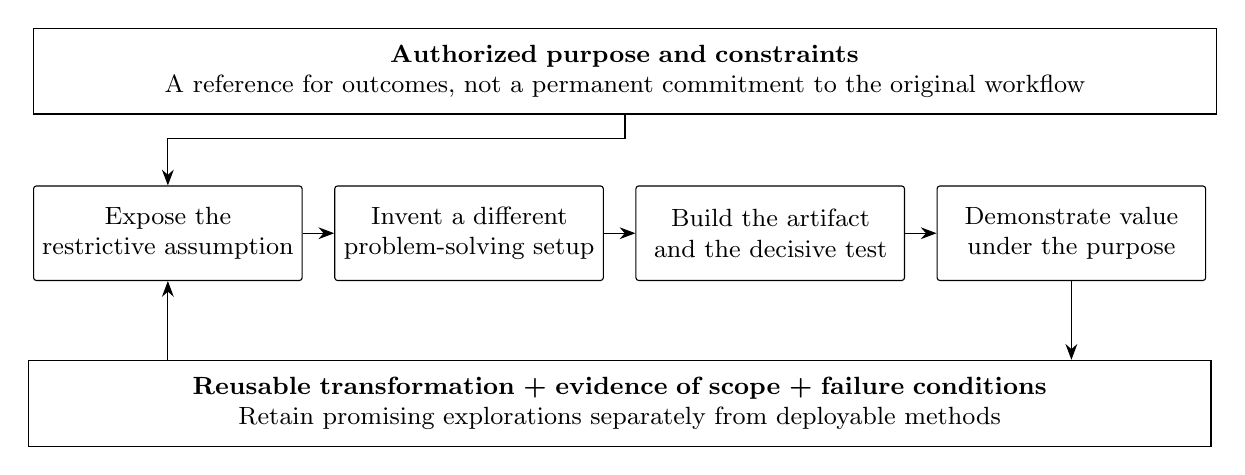
\begin{tikzpicture}[font=\small, node distance=6mm and 4mm, >={Stealth[length=2mm]}, box/.style={draw,rounded corners=1pt,align=center,minimum height=12mm,text width=32mm,inner sep=3pt}]
\node[draw,align=center,text width=146mm,inner sep=6pt] (intent) {\textbf{Authorized purpose and constraints}\\A reference for outcomes, not a permanent commitment to the original workflow};
\node[box,below=9mm of intent.south west,anchor=north west] (diagnose) {Expose the\\restrictive assumption};
\node[box,right=of diagnose] (invent) {Invent a different\\problem-solving setup};
\node[box,right=of invent] (test) {Build the artifact\\and the decisive test};
\node[box,right=of test] (demonstrate) {Demonstrate value\\under the purpose};
\draw[->] (diagnose)--(invent);\draw[->] (invent)--(test);\draw[->] (test)--(demonstrate);
\draw[->] (intent.south) -- ++(0,-3mm) -| (diagnose.north);
\coordinate (rowbottom) at ($(diagnose.south)!0.5!(demonstrate.south)$);
\node[draw,below=10mm of rowbottom,align=center,text width=146mm,inner sep=6pt] (memory) {\textbf{Reusable transformation + evidence of scope + failure conditions}\\Retain promising explorations separately from deployable methods};
\draw[->] (demonstrate.south) -- (demonstrate.south |- memory.north);
\draw[->] (diagnose.south |- memory.north) -- (diagnose.south);
\end{tikzpicture}
\caption{The proposed architecture makes formulation change the creative center. Evidence is both a product of invention and the basis for deciding what deserves reuse.}
\label{fig:architecture}
\end{figure}

\section{Demonstration: did the change matter, and for the right reason?}
\label{sec:demonstration}
A transformational claim has three logically separate obligations: serve the authorized purpose, outperform an appropriate reference after costs, and support the attribution to a structural change. An impressive score alone settles none of them completely.

\subsection{The purpose bridge}
The bridge checks the original outcome, not merely the transformed procedure's internal target. Replacing a difficult scientific question with an easier conjecture is not a solution unless the conjecture actually advances the authorized research objective. A simulator-only result is not an operational result. A report with fewer inconvenient cases is not a more accurate report.

This does not demand that every useful change reproduce the old artifact. When the artifact is an instrumental means, an authorized transformation may replace it. What must remain comparable is the relevant user outcome. Where that outcome cannot be specified without further interaction, purpose discovery and stakeholder clarification become part of the work, with their costs and amendments visible.

\subsection{Structural attribution, not a weak-baseline victory}
A strong comparison includes a within-frame optimizer, a resource-matched unrestricted method with the same permitted tools, and an ablation that removes the specific proposed transformation while preserving the remaining implementation as far as possible. Giving a transformed candidate an intervention API while hiding the API from an unrestricted baseline would confound formulation discovery with unequal access.

At least three distinct statements should be reported. \emph{Observed improvement}: the candidate outperformed named baselines. \emph{Mechanism evidence}: a targeted ablation or experiment supports the role of the changed restriction. \emph{Certified ceiling escape}: an upper bound on the old frame is exceeded. The last is strongest and often unavailable. Success against a handful of workflows does not establish it.

A human-designed alternative frame is also useful as a diagnostic control. If a system performs well when given the frame but never discovers it, realization is not the bottleneck; formulation discovery is. That control is an achievable reference, not a mathematical upper bound. Separately, a baseline allowed to search for transformations tests whether the proposed discovery architecture adds value beyond the general instruction and tools.

\subsection{Count the whole transformation}
Report a cost vector, including model calls, tokens, tool time, elapsed time, human effort, data acquisition, and external resources. The lifecycle cost is
\begin{equation}
C_{\mathrm{life}}=C_{\mathrm{search}}+C_{\mathrm{build}}+C_{\mathrm{confirm}}+C_{\mathrm{migrate}}
+\sum_{r=1}^{R}(C_{\mathrm{execute},r}+C_{\mathrm{verify},r}+C_{\mathrm{maintain},r}).\label{eq:cost}
\end{equation}
A compiled representation can be advantageous at large reuse horizon $R$ and inferior for one use. A faster online decision may conceal expensive preparation. The exact example in Section~\ref{sec:causal} reports interaction counts and a specified interaction-cost objective; it does not claim equal lifecycle cost for discovering its two formulations.

Construction can also buy \emph{evaluability}. Suppose an old process costs $e_0$ to execute and $v_0$ to verify per use. A new representation costs $K$ up front and changes these to $e_1,v_1$. In common cost units, its simple break-even condition is
\begin{equation}
R[(e_0+v_0)-(e_1+v_1)]>K.\label{eq:verification-economics}
\end{equation}
This is an accounting condition, not a claim that every certificate is cheap or complete. Its implication is important: a slightly more expensive producer can be better overall if it makes reliable checking substantially cheaper. Conversely, adding a checker that itself needs intensive checking may not help.

\subsection{Fresh confirmation and calibrated measurements}
The final candidate, model configuration, bridge, sampling unit, and comparison protocol are frozen before confirmation. Within-episode adaptation remains allowed; cross-episode learning must either be disabled or included in a larger, independently sampled evaluation episode. Different questions from the same book or tasks sharing one repository are not automatically independent replicates.

For bounded paired outcome differences, Appendix~\ref{app:statistics} supplies a conservative false-promotion rule across adaptively proposed candidates, derived from Hoeffding's inequality \citep{hoeffding1963inequalities}. Fresh data and explicit error accounting are necessary because repeated feedback can contaminate a holdout \citep{dwork2014adaptive}. Valid sequential methods can replace fixed sample sizes when their assumptions hold \citep{howard2021confidence}.

Statistical confidence in the wrong instrument remains confidence in the wrong instrument. Let $\widetilde J(\pi)$ be expected measured utility and suppose a justified calibration bound gives
\begin{equation}
|\widetilde J(\pi)-J_\I(\pi)|\leq\varepsilon
\quad\text{for both frozen policies in a comparison}.\label{eq:calibration}
\end{equation}
Then a lower confidence bound $L$ on measured gain supports only $L-2\varepsilon$ as a corresponding lower bound on true gain. A practical-margin claim therefore needs $L>\delta+2\varepsilon$. Appendix~\ref{app:statistics} gives the short proof and the extra accounting needed when calibration is itself estimated. This exposes the cost of an inadequate evaluator instead of hiding it behind many agreeing judges.

\subsection{Negative controls are evidence of discernment}
A system rewarded only for finding transformations can learn to narrate a new game in every task. The evaluation must include cases where the apparent restriction is genuinely required, the proposed intervention is uninformative, the setup cost cannot be recovered, or the attractive new metric ignores a necessary outcome. In those cases, declining the change can be the successful behavior.

Measure the rate of useful accepted changes together with harmful or invalid changes, missed opportunities, cost, and abstention. A system that rejects everything has not demonstrated transformational capability; a system that accepts everything has not demonstrated judgment. Both errors matter.

\section{The evaluator must be revisable, too}
\label{sec:evaluator}
A framework that permits the problem to change but permanently freezes an inadequate evaluator can recreate the very ceiling it seeks to escape. A judge may reward the syntax of a familiar proof rather than its validity, the format of a report rather than its usefulness, or the number of completed steps rather than the outcome. The evaluation instrument must therefore be an object of research.

However, allowing a candidate to replace its judge and immediately declare victory destroys the comparison. The solution is not to forbid measurement change; it is to separate the questions \emph{Is this a better instrument?} and \emph{Does the candidate improve the outcome under a valid instrument?}

\subsection{An accountable instrument-change protocol}
A proposed evaluator revision states what the old instrument misses, supplies independent evidence for that diagnosis, and specifies a replacement. Validation uses external outcome evidence or separately adjudicated cases, including counterexamples on which the old and new instruments disagree. Acceptance is controlled outside the candidate's own optimization path.

After a change, rescore both candidates under the common validated instrument, or use a validated bridge to common outcomes. Preserve the earlier scores and record a new measurement epoch. A new evaluator may vindicate a previously rejected method, but that is a new supported comparison, not a retroactive claim that the old experiment proved more than it did. Where no adequate outcome anchor exists, the result remains a conditional measurement claim or an unresolved research question.

This protocol does not assume that a finite calibration set proves universal evaluator validity. Domain shift, new output structures, and adversarial adaptation can invalidate the bound. Independent audit cases and explicit scope restrictions remain necessary. Cryptographic digests can bind records to bytes; they cannot establish semantic truth or data independence.

\subsection{Purpose discovery is different from goal substitution}
Scientific investigation often changes the question as evidence accumulates. The framework must permit that. An AI can discover that an initial question is underspecified, that a hidden tradeoff matters, or that a different outcome would better serve a stakeholder's actual need. Human--AI research workflows have explicitly studied such iterative refinement of experimental intent \citep{bauerle2026intentmaking}.

The distinction is authority and attribution. Clarifying a means within the existing charter can remain part of the same task. Revising a material end, scope, or permission requires an authorized amendment. Once the objective changes, report progress under the new charter and explain its relationship to the old one. Do not compare incomparable scalar scores and call the difference an improvement.

\thesisbox{\textbf{Preserve the purpose, not every inherited proxy. Permit the question to evolve, but keep the authority and the evidence for that evolution visible.}}

\section{A research program that can falsify the thesis}
\label{sec:experiments}
The exact study establishes that formulation-dependent limits exist in a specified model. It does not establish that LLMs can reliably diagnose or escape such limits in unfamiliar environments. That is the empirical target.

\subsection{Task families with real opportunities and real traps}
A useful evaluation should sample mechanisms, not merely paraphrases. Table~\ref{tab:benchmarks} specifies proposed families. These are research designs, not completed benchmark results.
\begin{table}[htbp]
\centering\small
\caption{Proposed formulation-change evaluation families. Each requires a genuine opportunity, a matched negative control, and a common authorized outcome.}
\label{tab:benchmarks}
\begin{tabularx}{\linewidth}{@{}P{.16\linewidth}YYY@{}}
\toprule
Family & Opportunity & Negative control & Outcome evidence \\
\midrule
Representation & Discover a structure, invariant, or abstraction that reduces search & The proposed simplification discards a required distinction & Correctness, proof obligations, runtime, and total search cost \\
Information & Design a discriminating observation or experiment & No informative authorized intervention exists & Identification or decision quality under known or adjudicated outcomes \\
Coordination & Redesign avoidable dependencies or conflicting ownership & Dependencies are physically or contractually necessary & Valid completed artifacts, contention, duplication, and latency \\
Computer-mediated work & Replace recurring actions with an authorized reusable process & Low reuse, fragile automation, or forbidden side effects & Independent environment-state checks and lifecycle cost \\
Measurement & Replace a proxy that rejects a useful new solution form & The new judge merely lowers the standard & Agreement with independent purpose-grounded evidence and audited disagreements \\
\bottomrule
\end{tabularx}
\end{table}
For mathematical research, useful transformations may change a representation, search for a general construction rather than instances, introduce a lemma that reorganizes the proof, or find a reduction to a more tractable setting. A valid result and its novelty require separate checking. A computational pattern, a conjecture, a human-reviewed proof, and a formally checked proof must not share an undifferentiated success label.

For computer-mediated work, use resettable environments with independently inspectable final states. OSWorld provides a relevant precedent for evaluating actions in real computer environments \citep{xie2024osworld}; the proposed addition is to test discovery of a better workflow rather than only execution of a prescribed one. Broad access to keyboard-and-mouse interfaces is not evidence that all such work is automatable or that all outcomes are readily verifiable.

Include both synthetic tasks with known mechanisms and naturally arising tasks selected independently of the proposed method. Synthetic tasks permit complete checking but may reveal the designer's preferred escape route. Natural tasks test relevance but may not support a provable old-frame ceiling. Report these evidential differences rather than merging them into one transformational score.

\subsection{Baselines that isolate formulation discovery}
The primary comparison should keep the underlying model, external permissions, task exposure, and declared budgets matched. Include a tuned fixed-frame optimizer; an unrestricted agent explicitly allowed to question the formulation; a strong hand-engineered alternative; and an automated agent/workflow search method. ADAS, AFlow, and GEPA provide relevant families of such search baselines \citep{hu2024adas,zhang2024aflow,agrawal2025gepa}. A proposed system must earn its advantage over them, not merely over an unassisted first answer.

A factorial design crosses solver strength with formulation mutability. A further diagnostic supplies the discovered formulation to the old solver while holding other changes fixed. This separates the value of a new formulation, the ability to discover it, and the quality of its implementation. When a frame needs a compatible solver, test the combination and the interaction rather than assuming additive effects.

Cross initial instructions as well: present the same charter with a strongly suggested inherited workflow and with a neutral description. This helps distinguish resistance to prompt anchoring from discovery of a transferable mechanism. All methods must see the same authorized opportunities; a baseline should not be denied tools just to make it look frame-bound.

\subsection{Primary claims and disconfirming outcomes}
\paragraph{H1: useful formulation discovery.}
At matched lifecycle budget over a declared horizon, the proposed discovery process improves purpose-grounded outcomes on fresh task families relative to strong unrestricted discovery baselines. The claim is not supported if the gain disappears after counting search, setup, verification, or extra information access.

\paragraph{H2: structural attribution.}
The identified restriction explains a material part of the gain. Removing the transformation while retaining comparably tuned surrounding components reduces the advantage, and a mechanism-discriminating test behaves as predicted. The claim is weakened if a simpler unchanged-frame strategy matches the result at the same cost.

\paragraph{H3: selective reframing.}
The system changes genuinely removable restrictions more often than it changes required ones, while preserving material outcomes. Success requires useful changes as well as correct rejection; a policy of universal refusal does not qualify.

\paragraph{H4: transfer of reformulation skill.}
A discovery policy trained on donor families produces better transformations on held-out mechanism families from matched starting agents and archives. The claim is not supported by memorizing named transformations, transferring exact answers, or reusing a superior initialized solver without improving discovery.

\paragraph{H5: evaluator correction without self-approval.}
Independently validated instrument changes reveal genuine purpose-grounded improvements without increasing acceptance of known-invalid outcomes beyond the registered tolerance. The claim fails if gains occur only on the candidate's preferred judge or require suppressing contrary evidence.

\subsection{The correct unit of replication}
A task result supports an instance claim. A reusable formulation needs fresh instances. A policy that claims to learn how to discover formulations needs independent \emph{discovery campaigns}: matched initial resources, a development phase, finalist selection, and an untouched terminal evaluation. Hundreds of tasks inside one campaign do not create hundreds of independent demonstrations that the discovery policy improved.

Freeze model versions and initial memories where possible, record provider drift where not, blind adjudicators to expected winners, retain failed candidates, and account for all confirmatory attempts. For interventions in shared environments, randomize at an appropriate unit and model interference; two live runs are not paired counterfactual worlds merely because they have the same task title.

\section{Continuous discovery: accumulating ways to change the game}
\label{sec:continuous}
\subsection{Retain mechanisms with their conditions}
The durable memory should not say only ``this worked.'' It should retain the restriction encountered, the transformation attempted, the evidence supporting its mechanism, its prerequisites, its construction costs, its failure conditions, and the scope of its outcome claim. The same idea can succeed at a long reuse horizon and fail at a short one. A representation can be effective on reliable inputs and harmful on noisy ones.

Keep exploratory alternatives separate from deployable methods. Failure can be a useful stepping stone, but it is not authorization. A router that chooses among archived transformations is itself a policy: independently successful components do not guarantee that the router selects or composes them correctly. Revalidate significant changes to the model, environment, checker, or shared state.

\subsection{Learn the process of reframing}
Let $\eta$ be a discovery policy and $Z$ a fresh campaign initialization drawn from $\mathcal Q$. After discovery budget $B$, the policy returns a formulation-and-solver pair $(\widehat F,\widehat\pi)$. Let $W(\eta,Z,B)$ be a preregistered campaign outcome based on fresh terminal evaluations, material constraints, and costs. The meta-level target is
\begin{equation}
J_{\mathrm{reframe}}(\eta)=\E_{Z\sim\mathcal Q}[W(\eta,Z,B)].\label{eq:meta}
\end{equation}
Improving $\eta$ means increasing this quantity under matched conditions, not producing one impressive descendant. Cross old and new discovery policies with old and new initial task agents. A changed policy that helps only after inheriting a superior artifact has not thereby demonstrated better independent formulation discovery.

This is where meta-strategic and transformational intelligence meet. The system can learn which questions expose brittle assumptions, which experiments cheaply discriminate possibilities, which partial transformations are worth preserving, and which combinations deserve joint tests. The discovery process is editable; its claimed improvement still requires fresh campaign evidence. Prior work on self-modifying agents and meta-agents makes this a concrete comparison target rather than a claim of an untouched field \citep{zhang2025dgm,zhang2026hyperagents}.

\subsection{Compounding is a hypothesis, not a slogan}
A successful transformation can lower the cost of producing or validating later transformations. A reusable representation might make future tasks easier to express; a reliable checker might make more candidate ideas affordable to test. This creates a possible feedback mechanism. It does not imply exponential growth, universal transfer, or monotonic improvement.

For a fixed bounded objective, infinitely many gains of a fixed positive size are impossible. ``Continuously discovers'' means an enduring capacity to search, test, retain, adapt, and sometimes stop. Evidence can compound as knowledge of scope and failure, even when the current best performance does not improve. Changes to the task distribution or objective create new claims, not permission to concatenate incompatible scores into an acceleration curve.

\section{Relationship to prior work}
\label{sec:related}
\paragraph{Transforming conceptual spaces.}
Boden distinguishes combining familiar ideas, exploring a conceptual space, and changing the space so that previously unavailable ideas can be generated \citep{boden1998creativity}. The present formulation is close in spirit. Its added emphasis is an operational link between a changed problem-solving setup, authorized outcomes, resource use, and evidence of the change's contribution. It is not a new name for all creativity.

\paragraph{Metareasoning, languages, and open-ended tasks.}
Metareasoning studies which computations are worth performing \citep{hay2012selecting}. DreamCoder learns abstractions and languages that support program search \citep{ellis2020dreamcoder}. POWERPLAY jointly searches new tasks and solver modifications \citep{schmidhuber2011powerplay}, while POET co-develops environments and solutions with transfer between them \citep{wang2019poet}. These are important precedents for making problem structure and discovery processes editable. Here the central application is reformulation in service of a declared external purpose; inventing an interesting new task alone does not establish that purpose was served.

\paragraph{Critique and automated agent design.}
Debate and tool-grounded critique motivate scrutiny that can expose checkable errors \citep{irving2018debate,gou2023critic}. Earlier self-correction experiments also show why improvement cannot be assumed merely from requesting another pass \citep{huang2023selfcorrect}. ADAS, AFlow, and GEPA search agent designs, workflows, or prompts \citep{hu2024adas,zhang2024aflow,agrawal2025gepa}. Depending on their realized behavior, such systems may discover transformational changes; the categories are not defined by the system's brand or optimization algorithm.

\paragraph{Algorithm discovery and self-improvement.}
AlphaEvolve combines model-generated code, evaluators, and evolutionary search in algorithmic and scientific settings \citep{novikov2025alphaevolve}. The Darwin G\"odel Machine explores empirically evaluated self-modifications, and Hyperagents makes the meta-level modification procedure editable \citep{zhang2025dgm,zhang2026hyperagents}. These are direct precedents for executable invention and improving improvement procedures. The additional question asked here is whether a gain arose from overcoming a particular formulation restriction, whether it survives strong unrestricted controls, and how to validate a necessary change to the evaluation instrument itself.

\paragraph{Causality and adaptive evidence.}
The exact example draws on ordinary causal semantics \citep{pearl2009causal}; its role is to make the limits of a frame analytically visible. The confirmation protocol applies standard concentration and adaptive-data principles \citep{hoeffding1963inequalities,dwork2014adaptive,howard2021confidence}. Neither the example nor the statistical appendix is claimed as a new general theory in those fields. The intended contribution is the way these pieces turn a broad aspiration into distinguishable, testable claims.

\clearpage
\section{The decisive research challenge}
\label{sec:conclusion}
The hard part is not getting an AI to describe a clever reframing. It is getting it to recognize a consequential restriction in an unfamiliar task, construct a feasible alternative, and produce evidence that the alternative serves the user's purpose better after its full costs are paid.

Four obstacles deserve priority. Assumption discovery must distinguish conventions from real constraints. Candidate generation must reach beyond cosmetic edits without making search prohibitively expensive. Demonstration must remain meaningful when the representation or evaluation instrument changes. Transfer must be shown across mechanisms, not inferred from a collection of memorable successes. The proposed architecture does not remove these difficulties; it makes them experimentally separable.

A compelling next result would combine a newly encountered natural task, a documented diagnosis of its restrictive formulation, an executable alternative, a strong same-permission baseline, an independently checked outcome bridge, and a fresh replication. A still stronger result would show that a learned discovery policy repeatedly produces such transformations across unfamiliar task families. Either result could fail in informative ways, and neither should be replaced by an architecture diagram or an eloquent self-assessment.

The first draft of a problem is not necessarily the best place to spend the next million units of intelligence. Sometimes the right investment is to make the original search easier. Sometimes it is to discover that the important information must be acquired differently, that the work can be organized around different dependencies, or that a recurring task can be made unnecessary. Those are not merely better answers. They are better conditions for producing useful answers and actions.

\thesisbox{\textbf{The research objective is an AI that does not merely become better at solving the problems it is given. It learns when those problems have been unnecessarily constrained, discovers a better game to play, and demonstrates---under the purpose that justified the work---that changing the game was the right move.}}

\section*{Research status, reproducibility, and limitations}
This manuscript reports an operational framework, analytic arguments, an exact finite synthetic computation, and a proposed empirical program. The companion implementation reproduces Table~\ref{tab:exact}, verifies Bellman and closed-form agreement, executes negative controls, and checks selected mathematical boundary conditions. It uses no frontier-model calls. It does not establish autonomous discovery of the model family or transformation, general transformational intelligence, real-world deployment performance, or external peer review. A successful test suite checks specified computations; it does not establish that all scientific or operational assumptions hold. Detailed reproduction instructions and the claim--evidence register accompany the source.

\clearpage
\begingroup
\small
\urlstyle{same}
\setlength{\bibsep}{0.5em}
\begin{thebibliography}{20}
\bibitem[Agrawal et~al.(2025)]{agrawal2025gepa}
Lakshya A. Agrawal et~al.
\newblock {GEPA}: Reflective Prompt Evolution Can Outperform Reinforcement Learning.
\newblock arXiv:2507.19457, 2025.
\newblock \url{https://arxiv.org/abs/2507.19457}.

\bibitem[B{\"a}uerle et~al.(2026)]{bauerle2026intentmaking}
Alex B{\"a}uerle et~al.
\newblock Intentmaking and Sensemaking: Human Interaction with {AI}-Guided Mathematical Discovery.
\newblock arXiv:2605.05921, 2026.
\newblock \url{https://arxiv.org/abs/2605.05921}.

\bibitem[Boden(1998)]{boden1998creativity}
Margaret A. Boden.
\newblock Creativity and artificial intelligence.
\newblock \emph{Artificial Intelligence}, 103(1--2):347--356, 1998.
\newblock \url{https://doi.org/10.1016/S0004-3702(98)00055-1}.

\bibitem[Dwork et~al.(2014)]{dwork2014adaptive}
Cynthia Dwork, Vitaly Feldman, Moritz Hardt, Toniann Pitassi, Omer Reingold, and Aaron Roth.
\newblock Preserving Statistical Validity in Adaptive Data Analysis.
\newblock arXiv:1411.2664, 2014.
\newblock \url{https://arxiv.org/abs/1411.2664}.

\bibitem[Ellis et~al.(2020)]{ellis2020dreamcoder}
Kevin Ellis et~al.
\newblock {DreamCoder}: Growing generalizable, interpretable knowledge with wake-sleep {Bayesian} program learning.
\newblock arXiv:2006.08381, 2020.
\newblock \url{https://arxiv.org/abs/2006.08381}.

\bibitem[Gou et~al.(2023)]{gou2023critic}
Zhibin Gou, Zhihong Shao, Yeyun Gong, Yelong Shen, Yujiu Yang, Nan Duan, and Weizhu Chen.
\newblock {CRITIC}: Large Language Models Can Self-Correct with Tool-Interactive Critiquing.
\newblock arXiv:2305.11738, 2023.
\newblock \url{https://arxiv.org/abs/2305.11738}.

\bibitem[Hay et~al.(2012)]{hay2012selecting}
Nicholas Hay, Stuart Russell, David Tolpin, and Solomon Eyal Shimony.
\newblock Selecting Computations: Theory and Applications.
\newblock arXiv:1207.5879, 2012.
\newblock \url{https://arxiv.org/abs/1207.5879}.

\bibitem[Hoeffding(1963)]{hoeffding1963inequalities}
Wassily Hoeffding.
\newblock Probability inequalities for sums of bounded random variables.
\newblock \emph{Journal of the American Statistical Association}, 58(301):13--30, 1963.
\newblock \url{https://doi.org/10.1080/01621459.1963.10500830}.

\bibitem[Howard et~al.(2021)]{howard2021confidence}
Steven R. Howard, Aaditya Ramdas, Jon McAuliffe, and Jasjeet Sekhon.
\newblock Time-uniform, nonparametric, nonasymptotic confidence sequences.
\newblock \emph{The Annals of Statistics}, 49(2):1055--1080, 2021.
\newblock \url{https://arxiv.org/abs/1810.08240}.

\bibitem[Hu et~al.(2024)]{hu2024adas}
Shengran Hu, Cong Lu, and Jeff Clune.
\newblock Automated Design of Agentic Systems.
\newblock arXiv:2408.08435, 2024.
\newblock \url{https://arxiv.org/abs/2408.08435}.

\bibitem[Huang et~al.(2023)]{huang2023selfcorrect}
Jie Huang, Xinyun Chen, Swaroop Mishra, Huaixiu Steven Zheng, Adams Wei Yu, Xinying Song, and Denny Zhou.
\newblock Large Language Models Cannot Self-Correct Reasoning Yet.
\newblock arXiv:2310.01798, 2023.
\newblock \url{https://arxiv.org/abs/2310.01798}.

\bibitem[Irving et~al.(2018)]{irving2018debate}
Geoffrey Irving, Paul Christiano, and Dario Amodei.
\newblock {AI} safety via debate.
\newblock arXiv:1805.00899, 2018.
\newblock \url{https://arxiv.org/abs/1805.00899}.

\bibitem[Novikov et~al.(2025)]{novikov2025alphaevolve}
Alexander Novikov et~al.
\newblock {AlphaEvolve}: A coding agent for scientific and algorithmic discovery.
\newblock arXiv:2506.13131, 2025.
\newblock \url{https://arxiv.org/abs/2506.13131}.

\bibitem[Pearl(2009)]{pearl2009causal}
Judea Pearl.
\newblock Causal inference in statistics: An overview.
\newblock \emph{Statistics Surveys}, 3:96--146, 2009.
\newblock \url{https://ftp.cs.ucla.edu/pub/stat_ser/r350.pdf}.

\bibitem[Schmidhuber(2011)]{schmidhuber2011powerplay}
J{\"u}rgen Schmidhuber.
\newblock {POWERPLAY}: Training an Increasingly General Problem Solver by Continually Searching for the Simplest Still Unsolvable Problem.
\newblock arXiv:1112.5309, 2011.
\newblock \url{https://arxiv.org/abs/1112.5309}.

\bibitem[Wang et~al.(2019)]{wang2019poet}
Rui Wang, Joel Lehman, Jeff Clune, and Kenneth O. Stanley.
\newblock Paired Open-Ended Trailblazer ({POET}): Endlessly Generating Increasingly Complex and Diverse Learning Environments and Their Solutions.
\newblock arXiv:1901.01753, 2019.
\newblock \url{https://arxiv.org/abs/1901.01753}.

\bibitem[Xie et~al.(2024)]{xie2024osworld}
Tianbao Xie et~al.
\newblock {OSWorld}: Benchmarking Multimodal Agents for Open-Ended Tasks in Real Computer Environments.
\newblock arXiv:2404.07972, 2024.
\newblock \url{https://arxiv.org/abs/2404.07972}.

\bibitem[Zhang et~al.(2024)]{zhang2024aflow}
Jiayi Zhang et~al.
\newblock {AFlow}: Automating Agentic Workflow Generation.
\newblock arXiv:2410.10762, 2024.
\newblock \url{https://arxiv.org/abs/2410.10762}.

\bibitem[Zhang et~al.(2025)]{zhang2025dgm}
Jenny Zhang, Shengran Hu, Cong Lu, Robert Lange, and Jeff Clune.
\newblock {Darwin G{\"o}del Machine}: Open-Ended Evolution of Self-Improving Agents.
\newblock arXiv:2505.22954, 2025.
\newblock \url{https://arxiv.org/abs/2505.22954}.

\bibitem[Zhang et~al.(2026)]{zhang2026hyperagents}
Jenny Zhang, Bingchen Zhao, Wannan Yang, Jakob Foerster, Jeff Clune, Minqi Jiang, Sam Devlin, and Tatiana Shavrina.
\newblock {Hyperagents}.
\newblock arXiv:2603.19461, 2026.
\newblock \url{https://arxiv.org/abs/2603.19461}.

\end{thebibliography}
\endgroup

\clearpage
\appendix
\section{Exact study: model, optimization, and reproduction}
\label{app:study}
\subsection{What is supplied, and what is computed}
The experiment supplies the two structural hypotheses in Equations~\eqref{eq:cause}--\eqref{eq:confounded}, the uniform prior, independent fresh latent bits, the action set, and the loss. These are investigator choices. The computation finds an optimal policy within this supplied finite-horizon decision problem and checks it by exhaustive execution. It does not infer the hypothesis space from natural language, invent an intervention API, or discover that causal experimentation is useful without that setup.

For passive observation the implementation returns $Y$; because $X=Y$ almost surely in both worlds, this encodes the entire observed pair without losing information. For an intervention the chosen $X$ is already known, so the returned $Y$ likewise supplies the full observable response. The latent bit is never exposed to the policy. A new independent bit is generated at each step, while the hidden world remains fixed within an episode.

Let $p=\Prob(\Theta=c\mid h)$ be the posterior after history $h$, let $r$ be the remaining query budget, and let $q_a(y\mid p)$ be the predictive probability of response $y$ under action $a$. If $p_{a,y}$ is the corresponding Bayesian posterior, the optimal expected loss satisfies
\begin{align}
V_0(p)&=\min\{p,1-p\},\nonumber\\
V_r(p)&=\min\left\{p,1-p,\min_{a\in A_F}\left[\lambda+\sum_{y\in\{0,1\}}q_a(y\mid p)V_{r-1}(p_{a,y})\right]\right\}.
\label{eq:bellman}
\end{align}
Zero-probability branches are omitted. The first two terms choose a world and stop; the remaining terms perform an authorized query and continue. The companion code uses exact rational arithmetic and memoization. It resolves equal losses in favor of fewer expected queries, then by a deterministic action ordering. An empty action set still permits stopping.

\subsection{Why the simple active policy is optimal here}
Passive observations do not change $p$. The two interventions are equivalent up to relabeling the returned bit: a response disagreeing with the imposed $X$ proves world $f$, and a matching response increases the posterior probability of $c$. Once a disagreement occurs, additional queries cannot improve identification. Before a disagreement, every useful query has the same information structure. For zero query cost, using the available interventions therefore weakly dominates spending a step observing or stopping early. Starting from $p=1/2$, the resulting policy is exactly the one in Section~\ref{sec:causal}.

For nonnegative query cost, all uncertainty remains on a single matching-response branch. A deterministic policy is consequently characterized, up to equivalent action relabeling, by a maximum number $k$ of interventions before stopping on that branch. Randomization cannot improve expected loss beyond the best deterministic choice. Its loss is
\begin{equation}
\mathcal L_\lambda(k)=2^{-(k+1)}+\lambda\left(\frac{k}{2}+1-2^{-k}\right),\qquad 0\leq k\leq m.
\label{eq:caploss}
\end{equation}
The marginal change from allowing one more intervention is
\begin{equation}
\mathcal L_\lambda(k+1)-\mathcal L_\lambda(k)
=-2^{-(k+2)}+\lambda\left(\frac12+2^{-(k+1)}\right).
\label{eq:threshold}
\end{equation}
It is negative exactly when $\lambda<1/(2^{k+1}+2)$. The thresholds decrease with $k$, so they identify the optimal cap directly. Bellman recursion and this independent closed-form calculation agree in the released computations.

\begin{table}[htbp]
\centering\small
\caption{Exact cost-sensitive results with at most twelve queries. Query cost is measured in units of identification error. Setup, model acquisition, and deployment costs are not included in this illustrative loss. At an exact tie the lower-query policy is selected.}
\label{tab:cost}
\begin{tabular}{@{}rrrrr@{}}
\toprule
Cost $\lambda$ & Selected cap & Accuracy & Expected queries & Total loss \\
\midrule
$0$ & 12 & $8191/8192$ & $28671/4096$ & $1/8192$ \\
$1/256$ & 7 & $255/256$ & $575/128$ & $703/32768$ \\
$1/64$ & 5 & $63/64$ & $111/32$ & $143/2048$ \\
$1/8$ & 2 & $7/8$ & $7/4$ & $11/32$ \\
$1/4$ & 0 & $1/2$ & $0$ & $1/2$ \\
$1$ & 0 & $1/2$ & $0$ & $1/2$ \\
\bottomrule
\end{tabular}
\end{table}
The $\lambda=1/4$ case has two optimal caps, zero and one. Selecting zero implements the stated tie rule; it does not claim uniqueness. The interaction count is an execution-cost measure, not a measurement of how much real-world effort would be required to formulate the causal models or build a trustworthy intervention environment.

\subsection{Exhaustive execution and negative controls}
For horizon $m$, the checker enumerates both worlds and every binary latent sequence of length $m$, for $2^{m+1}$ equally weighted traces. It executes the selected policy without exposing future bits. Early stopping leaves unused suffix bits; enumerating those suffixes preserves the correct probability mass. The calculation obtains error probability and expected query count directly from trajectories and checks their agreement with the Bellman value and the closed forms. No Monte Carlo confidence interval is needed for this finite enumeration.

The uninformative-action control deliberately changes the response kernel so that both hidden labels have the same law under every query. It is a separate synthetic identification task, not a claim that an intervention has no effect in the original causal model. The optimal policy then stops at the prior accuracy. The permission control instead preserves the original model but exposes only observation as authorized; a proposed frame containing interventions is rejected before execution. The unrestricted-baseline control uses the same full-action Bellman planner as the active comparison and therefore matches it exactly.

This example assumes a correct, complete two-hypothesis model; noiseless deterministic response in world $c$; faithful interventions; a specified prior; and independent latent draws. Hidden additional hypotheses, noisy interventions, drifting worlds, or misspecified priors require a new analysis. The result is exact under its assumptions, not a universal accuracy claim about causal investigation.

\section{Statistical confirmation and measurement error}
\label{app:statistics}
This appendix gives a transparent reference gate, not a new concentration inequality. It makes explicit what repeated, adaptively selected improvement claims require. The gate concerns a declared population and valid measurements; it does not certify every instance or every possible harm.

\subsection{A conditional guarantee across adaptive candidates}
At attempt $t$, freeze a candidate, a comparator, their initial states, a bounded evaluation score $S\in[0,1]$, a practical margin $\delta_t\geq0$, and a sample size $n_t$. Let $Y_{t,i}\in[-1,1]$ be the candidate-minus-comparator score difference on fresh paired episode $i$. The two runs within a pair need not be independent, but pairs are independent under the registered design. They must not contaminate each other's state. Write
\begin{equation}
\widehat\Delta_t=\frac1{n_t}\sum_iY_{t,i},\qquad
L_t=\widehat\Delta_t-\sqrt{\frac{2\log(1/\alpha_t)}{n_t}}.
\label{eq:lcb}
\end{equation}
The factor of two comes from the width-two range of paired differences. Using a width-one bound here would overstate precision.

\begin{theorem}[False-promotion control under fresh confirmation]
\label{thm:promotion}
Let $\Hist_{t-1}$ contain all information available before attempt $t$ draws its confirmation sample. Conditional on $\Hist_{t-1}$, suppose all choices above are fixed and the $Y_{t,i}$ are independent with common mean $\Delta_t$. Let deterministic allocations satisfy $\sum_{t\geq1}\alpha_t\leq\alpha$. Then accepting a score-improvement claim only when $L_t>\delta_t$ gives
\begin{equation}
\Prob\!\left(\exists t:\;L_t>\delta_t\ \text{and}\ \Delta_t\leq\delta_t\right)\leq\alpha.
\label{eq:familywise}
\end{equation}
Candidate generation may adapt to all earlier completed attempts. It may not adapt to its own current confirmation outcomes before the registered analysis.
\end{theorem}
\begin{proof}
Conditionally on $\Hist_{t-1}$, Hoeffding's inequality bounds
\[
\Prob\!\left(\widehat\Delta_t-\Delta_t>
\sqrt{2\log(1/\alpha_t)/n_t}\mid\Hist_{t-1}\right)\leq\alpha_t.
\]
A false acceptance implies this event. Taking expectations and a countable union bound yields Equation~\eqref{eq:familywise}. Independence between separate attempts is unnecessary.
\end{proof}
This is a direct application of established concentration and multiplicity control \citep{hoeffding1963inequalities}. A convenient schedule is $\alpha_t=\alpha/[t(t+1)]$. When attempt $t$ supports $m_t$ separate prespecified claims, an elementary allocation is $\alpha_{t,j}=\alpha/[t(t+1)m_t]$. All attempts count, including failed ones and parallel candidates sharing the global claim. Renaming a project does not reset its error budget.

The theorem does not authorize repeatedly inspecting the fixed-$n$ bound and stopping as soon as it passes. A valid confidence sequence or a separately justified sequential design is needed for such stopping \citep{howard2021confidence}. A test set that repeatedly informs revisions is development data unless a valid adaptive-reuse procedure applies \citep{dwork2014adaptive}. Questions from one book, tasks from one shared environment, and descendants from one discovery campaign must not be counted as independent replicates merely because there are many of them.

\subsection{A precise measurement bridge}
Suppose the intended outcome is $U\in[0,1]$, while the evaluator returns $S\in[0,1]$. For each compared policy $\pi$, assume a separately justified calibration bound
\begin{equation}
\left|\E[S\mid\pi]-\E[U\mid\pi]\right|\leq\varepsilon.
\label{eq:biasassumption}
\end{equation}
Then the intended outcome gain satisfies
\begin{equation}
\Delta_U\geq\Delta_S-2\varepsilon.
\label{eq:bridgegain}
\end{equation}
This follows by writing the two expectation errors separately and taking their worst signs. With unequal bounds, replace $2\varepsilon$ by $\varepsilon_{\mathrm{candidate}}+\varepsilon_{\mathrm{comparator}}$. Thus $L_t-2\varepsilon>\delta_t$ is a sufficient performance gate for the intended gain under the calibration assumption. If calibration is itself only supported with failure probability at most $\gamma$, account for it separately; a union bound gives at most $\alpha+\gamma$ for these two types of erroneous claims. A shared, uniform calibration event and many separately estimated calibration events require different accounting.

Calibration on familiar outputs need not apply to a radically new output structure. A transformed representation can invalidate precisely the instrument used to evaluate it. The response is to investigate the measurement bridge, not to assign a convenient $\varepsilon$ or let model agreement stand in for calibration.

For a constructed arithmetic illustration, take total $\alpha=0.05$, the first attempt and one claim, so $\alpha_1=0.025$. With $n=2000$ and hypothetical observed mean gain $0.10$, Equation~\eqref{eq:lcb} gives $L\approx0.0392639$. A practical margin of $0.02$ passes on the score alone. With a separately justified $\varepsilon=0.01$ for each policy, the corrected bound is only $0.0192639$, which does not pass. These numbers are not observations from a frontier model or a calibration study; they illustrate why a precise score comparison may still be insufficient.

\subsection{Constraints and the limits of a mean improvement}
For a frozen strategy with no observed failures in $n$ independent Bernoulli episodes, the exact one-sided upper bound at error level $\beta$ is
\begin{equation}
p_{\mathrm{upper}}=1-\beta^{1/n}.
\label{eq:nofailures}
\end{equation}
It follows from $(1-p)^n=\beta$. For $n=2000$ and $\beta=0.025$, the bound is approximately $0.00184274$, not zero. The companion checks this arithmetic, not the existence of a failure-free operational system. Different constraints, attempts, and stopping rules require appropriate error accounting. Hard prohibitions should also be enforced by the environment rather than left to a statistical average.

Finite evidence cannot generally prove universal correctness without additional structure. If two policies agree on all tested inputs and differ on an untested input, the retained observations alone do not decide which is correct there. Formal proofs, sampling assumptions, and controlled exposure can support different scoped conclusions. None should be replaced by the claim that enough agreeing models eliminate all remaining assumptions.

\section{From a better summary to a better way of understanding}
\label{app:book}
The motivating book example is useful because it forces the framework to distinguish a genuinely new route from a silent change in the assignment. The following is a prospective protocol, not a report of completed reader experiments.

\subsection{Two legitimate charters, two different freedoms}
In a \emph{fixed-artifact charter}, the user needs a faithful summary of a particular edition, for a specified audience and purpose, within a strict length and format. The system may change how it reads, represents, drafts, and checks. It may not replace the requested summary with a longer document or an interactive product and declare success. An argument graph can be an internal transformation while the final artifact remains unchanged.

In an \emph{understanding charter}, the user instead authorizes a broader objective: reliably understand the book's central argument and use it in a specified class of decisions, within an attention budget. A static summary is one possible means. A source-grounded question interface, an adaptive explanation, or a small set of discriminating questions may be permissible alternatives. The freedom must be real and declared; the system cannot infer consent merely because another product sounds more sophisticated.

This distinction applies transformational intelligence to the initial request itself. It asks whether the summary is the user's end or the first proposed route to that end. When this is unresolved, clarification is an information-gathering action, not an excuse to evade a fully specified task.

\subsection{Three competing formulations}
The first formulation generates a summary and then uses source-grounded challenge, adjudication, and revision. Each accepted criticism must identify a source location, a material discrepancy, and its relevance to the declared purpose. A summary necessarily omits much of a book; omission alone is not an error.

The second formulation builds a source-grounded representation of claims, dependencies, qualifications, and conclusions before drafting. The summary is produced from this structure, and proposed coverage failures are traced through it. The transformation hypothesis is that preserving dependencies before compression reduces losses that are difficult to discover afterward. The counterhypothesis is that the graph introduces extraction errors and overhead that outweigh its benefit. The structure is itself audited, not treated as ground truth.

The third formulation, allowed only under the broader charter, organizes the output around the reader's intended questions and decisions. It maintains traceable source support and explicitly tests whether the reader can distinguish the author's central claims from important qualifications and competing interpretations. The transformed artifact may be interactive, but success is still judged by authorized understanding, not by engagement, verbosity, or satisfaction with a confident interface.

\subsection{What would constitute a convincing result?}
Use complete, lawfully accessible sources with fixed editions. Establish central-content judgments independently of method identity, with disagreement retained. Compare the first two formulations at the same output-length limit and with full accounting for source processing and review. Under the broader charter, compare static and adaptive methods at a matched reader-attention budget and common outcome assessment. Randomize readers across conditions or use a counterbalanced design with new books to avoid learning carryover.

Separate evaluative questions used to design the method from fresh questions and tasks used to test it. Include misleading prompts, plausible but false criticisms, reasonable omissions, and books whose structure is ill suited to a simple argument graph. Use books or independently sampled reader--book episodes as appropriate experimental units; many questions about one book do not supply independent evidence of transfer across books. Control familiarity with the source and report reader-level and book-level variation.

A structural ablation supplies the new representation to the old producer, removes dependency information while preserving comparable token budget, and contrasts source inspection before versus after exposure to the initial summary. These interventions help distinguish the value of the representation from more context, more attention, or critic anchoring. The proposed mechanism is not established by observing that the final prose looks more organized.

A convincing claim is therefore not ``three models approved this summary.'' It is that a particular change to how understanding is produced improved a prespecified outcome on new sources or readers, at an acceptable total cost, while preserving the original purpose. A single repaired omission demonstrates an instance correction; a reproducible formulation advantage demonstrates something larger.

\section{Transformation records and claim discipline}
\label{app:records}
\subsection{The minimum useful transformation witness}
A reusable record needs more than a prompt and a winning score. Table~\ref{tab:witness} specifies the essential contents. A proposed record can contain unresolved fields; an accepted empirical claim cannot silently leave its comparison or evidence undefined.
\begin{table}[htbp]
\centering\small
\caption{A transformation witness binds a structural hypothesis to its authorized scope and evidence. These are record requirements, not completed deployment claims.}
\label{tab:witness}
\begin{tabularx}{\linewidth}{@{}P{.24\linewidth}Y@{}}
\toprule
Field & Required content \\
\midrule
Purpose & Original charter, material constraints, and any authorized amendment \\
Restriction & The inherited assumption, its provenance, why it may be unnecessary, and evidence that it is binding \\
Transformation & Executable construction, changed representation or protocol, prerequisites, and fallback \\
Bridge & How original outcomes and permissions are preserved; formal, empirical, or judgment-based scope \\
Falsifier & A predicted observation or intervention that would undermine the mechanism claim \\
Comparison & Strong baselines, matched opportunities, cost horizon, model identity, and tuning access \\
Confirmation & Frozen artifact identities, sampling unit, fresh evidence, uncertainty, and all failed attempts \\
Reuse conditions & Supported task family, maintenance requirements, failure cases, and retirement triggers \\
\bottomrule
\end{tabularx}
\end{table}
Artifact hashes establish byte identity only when computed from actual files. They do not prove when an artifact was frozen, whether evidence was independent, or whether the intended outcome was measured correctly. Those properties require a trustworthy experimental process. Exploration logs should preserve rejected and inconclusive candidates; a lineage containing only winners invites selection bias.

\subsection{What the present artifact establishes}
The passive-information ceiling and active closed forms are derived under explicit finite-model assumptions. The companion independently checks their instantiated arithmetic through Bellman recursion and exhaustive trace execution. The cost thresholds and complementary-edit example are analytic constructions with computational checks. The statistical gate is a standard conditional guarantee; its numerical example is illustrative. The discovery architecture, benchmark families, book protocol, and transfer hypotheses are proposed research, not measured performance.

The package includes the standalone manuscript, an editable bibliography, the standard-library Python experiment, unit tests, retained results, and build instructions. The reproduction commands are:
\begin{lstlisting}
python -m unittest -v
python frame_lab.py --out results
pdflatex -interaction=nonstopmode -halt-on-error Transformational_Intelligence.tex
pdflatex -interaction=nonstopmode -halt-on-error Transformational_Intelligence.tex
\end{lstlisting}
The LaTeX source embeds its bibliography and uses no external figure files. The separate \texttt{references.bib} is supplied for editing or integration into another publication workflow. The released results are deterministic under the stated finite model; reproducing them does not reproduce an autonomous transformational discovery campaign. A future such campaign must release its own initialized agent, discovery history, controlled confirmation process, resource account, and independently inspectable outcomes.

\end{document}
